\chapter{История беспилотных транспортных средств} \label{chapt1}

\section{<<Стэнфордская тележка>>} \label{sect_StanfordCart}

В 1960 году студент Стэнфордского университета Джеймс Адамс в рамках своей
научной работы создал прототип самоуправляемой тележки, которая в дальнейшем
стала известна, как <<Стэнфордская тележка>> \cite{Glukhov_history}.
Система имела четыре канала для сбора информации об окружающей среде, которых
было достаточно для её автономного передвижения. <<Органы осязания>> были
представлены гибкими проволоками (<<кошачьими усам>>), при соприкосновении с
которыми срабатывали тормоза и тележка меняла направление движения,
чтобы объехать препятствие. Устройство также имело дальномер, определяющий
расстояние до препятствия или стен, а также камеру, служившую машине
<<глазами>> (рисунок \ref{img:stanford_cart}). Ориентация системы в
пространстве обеспечивалась специальной навигационной системой, отсчитывающей
пройденный путь. Тележка приводилась в действие оператором, печатающим
указания в специальном коде на телетайпе.

\begin{figure}[ht] 
  \centering
  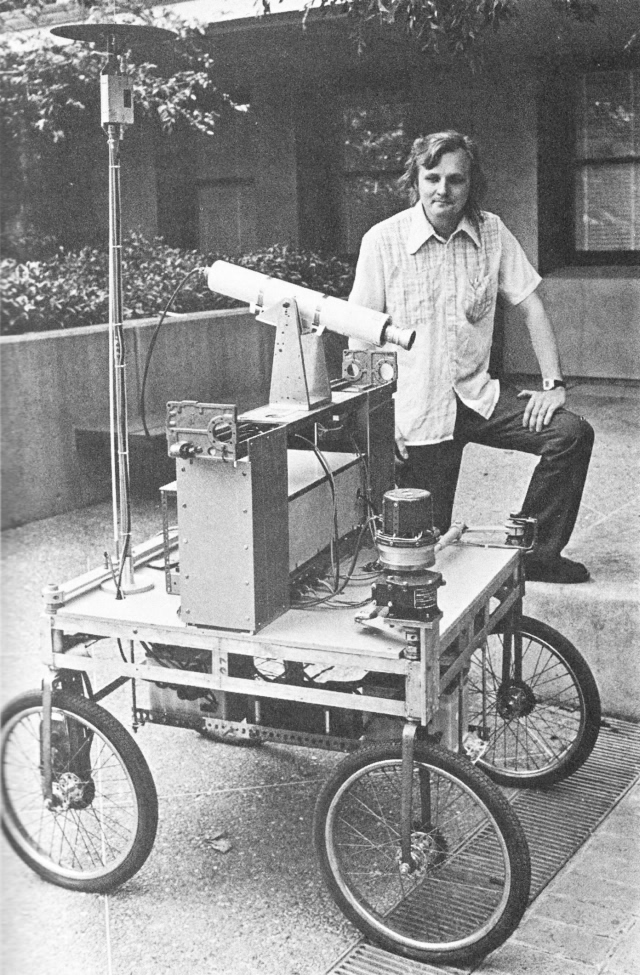
\includegraphics [scale=0.4] {stanford_cart}
  \caption{<<Стэнфордская тележка>>}
  \label{img:stanford_cart}
\end{figure}

В 1979 году Ханс Моравек перестраивает Стэнфордскую тележку, оснащая ее более
мощной системой технического зрения, и предпринимает ряд экспериментов по
трехмерному картографированию окружающей среды.

% Скопировано отсюда:
% http://www.lookatme.ru/mag/live/future-research/207541-sravnitelnaya-evolyutsiya-kak-razvivalis-roboty-i-chelovek

% Другие ссылки по теме:
% http://blog.skillfactory.ru/nauka-o-dannyh-data-science/vvedenie-v-mashinnoe-obuchenie/
% http://gagadget.com/science/21853-kak-razvivalis-bespilotnyie-avtomobili/
% https://strangernn.livejournal.com/1576029.html


%\newpage
%============================================================================================================================

\section{Aвтономный автомобиль Эрнста Дикманса} \label{sect_Dickmanns}

По сообщениям независимых экспертов первый полностью автономный автомобиль
был создан группой немецких ученных во главе с пионером робототехники
Эрнстом Дикмансом в 1980 году \cite{Dickmanns_vision}.
Для вычислений использовался мощный компьютер, который в то время был способен
уместиться лишь в грузовой фургон (рисунок \ref{img:dickmanns_car}).

\begin{figure}[ht] 
  \centering
  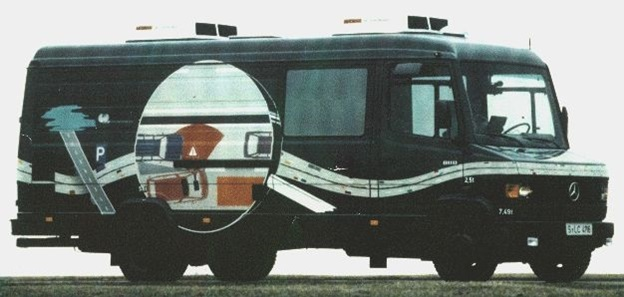
\includegraphics [scale=1.0] {dickmanns_car}
  \caption{Aвтономный автомобиль Эрнста Дикманса}
  \label{img:dickmanns_car}
\end{figure}

По данному проекту Дикмансом было опубликовано несколько научных работ, в 
которых детально описывались все технологии, применяемые в робомобиле. К ним 
можно отнести так называемый фильтр Калмана, имитацию саккадического движения 
глаз и механизмы параллельных вычислений. В некотором смысле эти технологии 
представляли собой модель машинного обучения, способную качественно оценивать 
всю окружающую обстановку.

% Скопировано отсюда:
% http://gagadget.com/science/21853-kak-razvivalis-bespilotnyie-avtomobili/

% Другие ссылки по теме:
% http://bespilot.com/info/istoriya
% https://geektimes.ru/post/274588/
% http://www.technoplusblog.ru/2017/10/blog-post.html


%\newpage
%============================================================================================================================

\section{Проект <<Прометей>>} \label{sect_Prometheus}

Автоконцерн Daimler-Benz обратил пристальное внимание на разработки Дикманса 
и запустил проект <<Прометей>>, основной целью которого было усовершенствование 
беспилотников и достижение беспрецедентной безопасности на дорогах. Проект 
взял старт в 1987 году и за время его существования (8 лет) было потрачено 
больше 1 млрд долларов \cite{MADI_GAZ}. <<Прометей>> вошел в историю как 
самый дорогой проект в сфере разработок робокаров ХХ века.
Однако инвестиции были потрачены не зря.

К середине 90-х миру были представлены два роботизированных беспилотника - 
VaMP (рисунок \ref{img:prometheus_vamp}) и VITA-2
(рисунок \ref{img:prometheus_vita2}). Они прошли успешное тестирование на 
полигоне в области Парижа, в процессе которого:

\begin{itemize}
  \item передвигались со скоростью до 130 км/ч полностью на автопилоте;
  \item самостоятельно перестраивались и меняли ряд;
  \item следили за дистанцией и передвижением других участников движения;
  \item обгоняли впереди идущие машины.
\end{itemize}

\begin{figure}[ht]
  {\centering
      \hfill
      \subbottom[List-of-Figures entry][VaMP\label{img:prometheus_vamp}]{%
          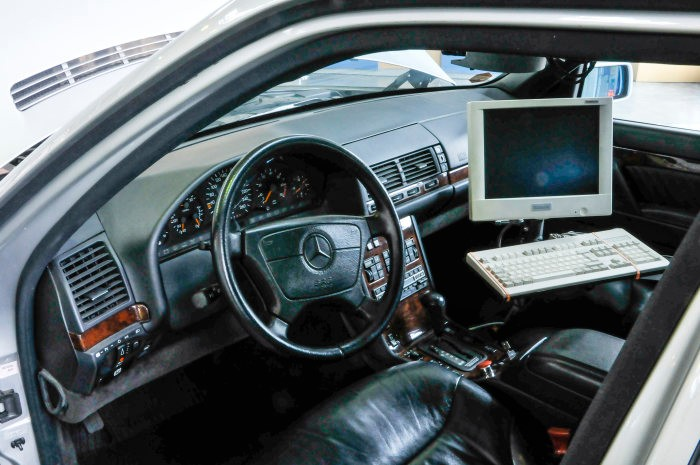
\includegraphics[width=0.44\linewidth]{prometheus_vamp}}
      \hfill
      \subbottom[VITA-2\label{img:prometheus_vita2}]{%
          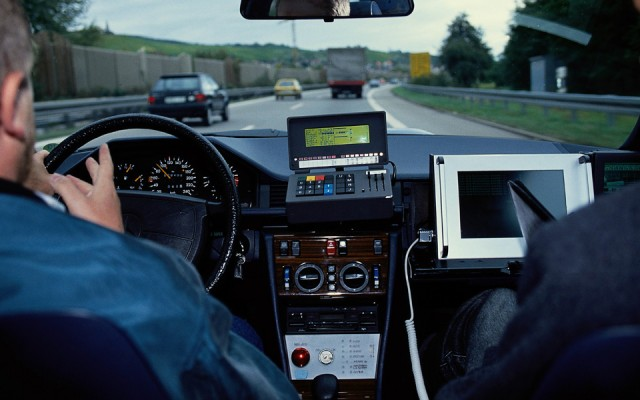
\includegraphics[width=0.47\linewidth]{prometheus_vita2}}
      \hfill
  }
  \caption{Автомобили проекта <<Прометей>>}
  \label{img:prometheus}
\end{figure}

Результатами проекта <<Прометей>> и разработками Дикманса воспользовались для 
серийного производства Mersedes-ов S-класса 1995 года. Эти машины были 
оснащены более продвинутой системой круиз-контроля, которая позволяла 
адаптироваться к средней скорости автомобильного потока и не нарушать дистанцию 
между авто.

% Скопировано отсюда:
% http://bespilot.com/info/istoriya

% Другие ссылки по теме:
% http://gagadget.com/science/21853-kak-razvivalis-bespilotnyie-avtomobili/
% https://geektimes.ru/post/274588/
% http://www.technoplusblog.ru/2017/10/blog-post.html


%\newpage
%============================================================================================================================

\section{Ссылки} \label{sect1_2}
Сошлёмся на библиографию.
Одна ссылка: \cite[с.~54]{Sokolov}\cite[с.~36]{Gaidaenko}.
Две ссылки: \cite{Sokolov,Gaidaenko}.
Много ссылок: %\cite[с.~54]{Lermontov,Management,Borozda} % такой «фокус» вызывает biblatex warning относительно опции sortcites, потому что неясно, к какому источнику относится уточнение о страницах, а bibtex об этой проблеме даже не предупреждает
\cite{Lermontov,Management,Borozda,Marketing,Constitution,FamilyCode,Gost.7.0.53,Razumovski,Lagkueva,Pokrovski,Sirotko,Lukina,Methodology,Encyclopedia,Nasirova,Berestova,Kriger}.
И~ещё немного ссылок:
\cite{Article,Book,Booklet,Conference,Inbook,Incollection,Manual,Mastersthesis,Misc,Phdthesis,Proceedings,Techreport,Unpublished}.
\cite{medvedev2006jelektronnye, CEAT:CEAT581, doi:10.1080/01932691.2010.513279,Gosele1999161,Li2007StressAnalysis, Shoji199895,test:eisner-sample,AB_patent_Pomerantz_1968,iofis_patent1960}

%Попытка реализовать несколько ссылок на конкретные страницы для стандартной реализации:[\citenum{Sokolov}, с.~54; \citenum{Gaidaenko}, с.~36].

%Несколько источников мультицитата (только в biblatex)
%\cites[vii--x, 5, 7]{Sokolov}[v"--~x, 25, 526]{Gaidaenko} поехали дальше

Ссылки на собственные работы:~\cite{vakbib1, confbib1}

Сошлёмся на приложения: Приложение \ref{AppendixA}, Приложение \ref{AppendixB2}.

Сошлёмся на формулу: формула \eqref{eq:equation1}.

Сошлёмся на изображение: рисунок \ref{img:knuth}.

%\newpage
%============================================================================================================================

\section{Формулы} \label{sect1_3}

Благодаря пакету \textit{icomma}, \LaTeX~одинаково хорошо воспринимает в качестве десятичного разделителя и запятую ($3,1415$), и точку ($3.1415$).

\subsection{Ненумерованные одиночные формулы} \label{subsect1_3_1}

Вот так может выглядеть формула, которую необходимо вставить в строку по тексту: $x \approx \sin x$ при $x \to 0$.

А вот так выглядит ненумерованая отдельностоящая формула c подстрочными и надстрочными индексами:
\[
(x_1+x_2)^2 = x_1^2 + 2 x_1 x_2 + x_2^2
\]

При использовании дробей формулы могут получаться очень высокие:
\[
  \frac{1}{\sqrt{2}+
  \displaystyle\frac{1}{\sqrt{2}+
  \displaystyle\frac{1}{\sqrt{2}+\cdots}}}
\]

В формулах можно использовать греческие буквы:
\[
\alpha\beta\gamma\delta\epsilon\varepsilon\zeta\eta\theta\vartheta\iota\kappa\lambda\\mu\nu\xi\pi\varpi\rho\varrho\sigma\varsigma\tau\upsilon\phi\varphi\chi\psi\omega\Gamma\Delta\Theta\Lambda\Xi\Pi\Sigma\Upsilon\Phi\Psi\Omega
\]

\def\slantfrac#1#2{ \hspace{3pt}\!^{#1}\!\!\hspace{1pt}/
  \hspace{2pt}\!\!_{#2}\!\hspace{3pt}
} %Макрос для красивых дробей в строчку (например, 1/2)
Для красивых дробей (например, в индексах) можно добавить макрос
\verb+\slantfrac+ и писать $\slantfrac{1}{2}$ вместо $1/2$.
%\newpage
%============================================================================================================================

\subsection{Ненумерованные многострочные формулы} \label{subsect1_3_2}

Вот так можно написать две формулы, не нумеруя их, чтобы знаки равно были строго друг под другом:
\begin{align}
  f_W & =  \min \left( 1, \max \left( 0, \frac{W_{soil} / W_{max}}{W_{crit}} \right)  \right), \nonumber \\
  f_T & =  \min \left( 1, \max \left( 0, \frac{T_s / T_{melt}}{T_{crit}} \right)  \right), \nonumber
\end{align}

Выровнять систему ещё и по переменной $ x $ можно, используя окружение \verb|alignedat| из пакета \verb|amsmath|. Вот так: 
\[
    |x| = \left\{
    \begin{alignedat}{2}
        &&x, \quad &\text{eсли } x\geqslant 0 \\
        &-&x, \quad & \text{eсли } x<0
    \end{alignedat}
    \right.
\]
Здесь первый амперсанд (в исходном \LaTeX\ описании формулы) означает выравнивание по~левому краю, второй "--- по~$ x $, а~третий "--- по~слову <<если>>. Команда \verb|\quad| делает большой горизонтальный пробел.

Ещё вариант:
\[
    |x|=
    \begin{cases}
    \phantom{-}x, \text{если } x \geqslant 0 \\
    -x, \text{если } x<0
    \end{cases}
\]

Кроме того, для  нумерованых формул \verb|alignedat|  делает вертикальное
выравнивание номера формулы по центру формулы. Например,  выравнивание компонент вектора:
\begin{equation}
 \label{eq:2p3}
 \begin{alignedat}{2}
{\mathbf{N}}_{o1n}^{(j)} = \,{\sin} \phi\,n\!\left(n+1\right)
         {\sin}\theta\,
         \pi_n\!\left({\cos} \theta\right)
         \frac{
               z_n^{(j)}\!\left( \rho \right)
              }{\rho}\,
           &{\boldsymbol{\hat{\mathrm e}}}_{r}\,+   \\
+\,
{\sin} \phi\,
         \tau_n\!\left({\cos} \theta\right)
         \frac{
            \left[\rho z_n^{(j)}\!\left( \rho \right)\right]^{\prime}
              }{\rho}\,
            &{\boldsymbol{\hat{\mathrm e}}}_{\theta}\,+   \\
+\,
{\cos} \phi\,
         \pi_n\!\left({\cos} \theta\right)
         \frac{
            \left[\rho z_n^{(j)}\!\left( \rho \right)\right]^{\prime}
              }{\rho}\,
            &{\boldsymbol{\hat{\mathrm e}}}_{\phi}\:.
\end{alignedat}
\end{equation}

Ещё об отступах. Иногда для лучшей <<читаемости>> формул полезно
немного исправить стандартные интервалы \LaTeX\ с учётом логической
структуры самой формулы. Например в формуле~\ref{eq:2p3} добавлен
небольшой отступ \verb+\,+ между основными сомножителями, ниже
результат применения всех вариантов отступа:
\begin{align*}
\backslash! &\quad f(x) = x^2\! +3x\! +2 \\
  \mbox{по-умолчанию} &\quad f(x) = x^2+3x+2 \\
\backslash, &\quad f(x) = x^2\, +3x\, +2 \\
\backslash{:} &\quad f(x) = x^2\: +3x\: +2 \\
\backslash; &\quad f(x) = x^2\; +3x\; +2 \\
\backslash \mbox{space} &\quad f(x) = x^2\ +3x\ +2 \\
\backslash \mbox{quad} &\quad f(x) = x^2\quad +3x\quad +2 \\
\backslash \mbox{qquad} &\quad f(x) = x^2\qquad +3x\qquad +2
\end{align*}


Можно использовать разные математические алфавиты:
\begin{align}
\mathcal{ABCDEFGHIJKLMNOPQRSTUVWXYZ} \nonumber \\
\mathfrak{ABCDEFGHIJKLMNOPQRSTUVWXYZ} \nonumber \\
\mathbb{ABCDEFGHIJKLMNOPQRSTUVWXYZ} \nonumber
\end{align}

Посмотрим на систему уравнений на примере аттрактора Лоренца:

\[ 
\left\{
  \begin{array}{rl}
    \dot x = & \sigma (y-x) \\
    \dot y = & x (r - z) - y \\
    \dot z = & xy - bz
  \end{array}
\right.
\]

А для вёрстки матриц удобно использовать многоточия:
\[ 
\left(
  \begin{array}{ccc}
  	a_{11} & \ldots & a_{1n} \\
  	\vdots & \ddots & \vdots \\
  	a_{n1} & \ldots & a_{nn} \\
  \end{array}
\right)
\]


%\newpage
%============================================================================================================================
\subsection{Нумерованные формулы} \label{subsect1_3_3}

А вот так пишется нумерованая формула:
\begin{equation}
  \label{eq:equation1}
  e = \lim_{n \to \infty} \left( 1+\frac{1}{n} \right) ^n
\end{equation}

Нумерованых формул может быть несколько:
\begin{equation}
  \label{eq:equation2}
  \lim_{n \to \infty} \sum_{k=1}^n \frac{1}{k^2} = \frac{\pi^2}{6}
\end{equation}

Впоследствии на формулы (\ref{eq:equation1}) и (\ref{eq:equation2}) можно ссылаться.

Сделать так, чтобы номер формулы стоял напротив средней строки, можно, используя окружение \verb|multlined| (пакет \verb|mathtools|) вместо \verb|multline| внутри окружения \verb|equation|. Вот так:
\begin{equation} % \tag{S} % tag - вписывает свой текст 
  \label{eq:equation3}
    \begin{multlined}
        1+ 2+3+4+5+6+7+\dots + \\ 
        + 50+51+52+53+54+55+56+57 + \dots + \\ 
        + 96+97+98+99+100=5050 
    \end{multlined}
\end{equation}

Используя команду \verb|\labelcref| из пакета \verb|cleveref|, можно
красиво ссылаться сразу на несколько формул
(\labelcref{eq:equation1,eq:equation3,eq:equation2}), даже перепутав
порядок ссылок \verb|(\labelcref{eq:equation1,eq:equation3,eq:equation2})|.

